% ======================================================================
%  Artigo SSCAD 2026 (template SBC)  -  Trabalho Final de CAD
% ----------------------------------------------------------------------
%  COMO COMPILAR (Overleaf, recomendado):
%   1. Crie um projeto em branco no Overleaf.
%   2. Faca upload de: este artigo.tex, sbc-template.sty, sbc.bst (ou use
%      o template oficial "SBC Conferences" do Overleaf) e das 3 imagens
%      bench_tempo.png, bench_speedup.png, bench_breakdown.png.
%   3. Compile com pdfLaTeX.
%  O sbc-template.sty esta em: SBC > Documentos Institucionais > Templates.
%  Limite SSCAD 2026: 12 paginas.
% ======================================================================
\documentclass[12pt]{article}

\usepackage{sbc-template}
\usepackage{graphicx}
\usepackage{url}
\usepackage[T1]{fontenc}
\usepackage[utf8]{inputenc}
\usepackage[brazil]{babel}

% Fallback: define o ambiente 'resumo' caso o sbc-template.sty carregado
% nao o defina (versoes antigas ou arquivos incorretos).
\makeatletter
\@ifundefined{resumo}{%
  \newenvironment{resumo}{%
    \renewcommand{\abstractname}{Resumo}%
    \begin{abstract}}{\end{abstract}}%
}{}
\makeatother
\usepackage{amsmath,amssymb}
\usepackage{booktabs}
\usepackage{listings}
\usepackage{xcolor}

\lstset{
  basicstyle=\ttfamily\scriptsize,
  keywordstyle=\color{blue!70!black},
  commentstyle=\color{green!40!black},
  breaklines=true,
  frame=single,
  language=C++,
  showstringspaces=false
}

\sloppy

\title{Aceleração em GPU do Cálculo Exato de Índices de Validação de
Agrupamentos: uma abordagem \emph{matrix-free} para os índices de
Dunn, Silhueta e Davies-Bouldin}

\author{Henrique M. M. Miranda, Cindy S. G. Rabelo,\\
Luiany G. Carvalho}

\address{Instituto de Informática -- Universidade Federal de Goiás (UFG)\\
  Goiânia -- GO -- Brasil
  \email{\{henrique.mendonca, cindy\_stephanie,
  luiany\}@discente.ufg.br}
}

\begin{document}

\maketitle

\begin{resumo}
A validação interna de agrupamentos (\emph{clustering}) por meio de índices
como Dunn, Silhueta e Davies-Bouldin exige o cálculo das distâncias
euclidianas par-a-par entre todos os pontos, com custo de tempo $O(N^2)$,
o que inviabiliza grandes volumes de dados em processadores sequenciais.
Este trabalho apresenta uma implementação \textbf{paralela e exata} desses
três índices em GPU com CUDA, adotando uma estratégia \emph{matrix-free}
que \textbf{não materializa} a matriz de distâncias $N\times N$: as
distâncias são recomputadas sob demanda dentro dos \emph{kernels}, reduzindo
a memória de $O(N^2)$ para $O(N\cdot D)$ e viabilizando $N=100.000$ pontos.
Comparando contra um \emph{baseline} em CPU (sequencial e paralelo via
OpenMP) numa mesma plataforma, obtivemos \emph{speed-up} de até
\textbf{24,9$\times$} (vs.\ CPU sequencial) e \textbf{24,5$\times$}
(vs.\ CPU OpenMP), com corretude validada em três camadas independentes
(caso analítico, \emph{scikit-learn} e equivalência CPU$\equiv$GPU).
\end{resumo}

\begin{abstract}
Internal validation of clustering through indices such as Dunn, Silhouette
and Davies-Bouldin requires computing pairwise Euclidean distances among all
points, with $O(N^2)$ time cost, which is prohibitive for large datasets on
sequential processors. This work presents a \textbf{parallel and exact}
GPU/CUDA implementation of these three indices using a \emph{matrix-free}
strategy that \textbf{does not materialize} the $N\times N$ distance matrix:
distances are recomputed on demand inside the kernels, reducing memory from
$O(N^2)$ to $O(N\cdot D)$ and enabling $N=100{,}000$ points. Against a CPU
\emph{baseline} (sequential and OpenMP-parallel) on the same platform, we
achieved speed-ups up to \textbf{24.9$\times$} (vs.\ sequential CPU) and
\textbf{24.5$\times$} (vs.\ OpenMP CPU), with correctness validated in three
independent layers (analytical case, \emph{scikit-learn}, and
CPU$\equiv$GPU equivalence).
\end{abstract}

% ======================================================================
\section{Introdução}
% ======================================================================

A análise de agrupamentos (\emph{clustering}) é uma técnica fundamental de
aprendizado não supervisionado, na qual objetos são particionados em grupos
de forma que elementos de um mesmo grupo sejam mais similares entre si do que
em relação aos demais. Algoritmos como K-Means e DBSCAN produzem partições,
mas \emph{toda} partição precisa ser \textbf{avaliada}: é necessário medir,
sem rótulos de referência, se os grupos obtidos são \emph{coesos}
internamente e \emph{bem separados} entre si. Essa medição é feita por
\textbf{índices internos de validação}, sendo três dos mais consagrados o
\textbf{Índice de Dunn}~\cite{dunn1974}, o \textbf{Coeficiente de
Silhueta}~\cite{rousseeuw1987} e o \textbf{Índice de
Davies-Bouldin}~\cite{davies1979}.

O gargalo computacional comum a Dunn e Silhueta é a necessidade de computar
as distâncias euclidianas \emph{par-a-par} entre todos os $N$ pontos,
resultando em complexidade de tempo $O(N^2 \cdot D)$, onde $D$ é a
dimensionalidade. Ao dobrar $N$, o esforço quadruplica; para dezenas ou
centenas de milhares de pontos, a validação sequencial em CPU torna-se
proibitiva. Essa limitação motiva o uso de arquiteturas de
\emph{paralelismo de dados massivo}, como as GPUs, nas quais milhares de
\emph{threads} executam simultaneamente a mesma operação simples (cálculo de
distância) sobre dados distintos.

O artigo de referência que fundamenta este projeto,
\emph{Parallel and scalable Dunn Index for the validation of big data
clusters}~\cite{ncir2021}, ataca o mesmo gargalo, porém com uma estratégia
distinta: distribui o cálculo em um \emph{cluster} de máquinas usando Apache
Spark e emprega \textbf{amostragem} (\emph{Sketch and Validate}) para
\textbf{aproximar} o índice em larga escala. O presente trabalho propõe uma
abordagem \textbf{complementar}: em vez de aproximar de forma distribuída,
calculamos os índices de forma \textbf{exata}, acelerados pelo paralelismo
de \emph{threads} de uma única GPU.

As principais contribuições deste trabalho são:
\begin{itemize}
  \item Uma implementação CUDA \textbf{exata} dos três índices (Dunn,
  Silhueta e Davies-Bouldin) com reduções em memória compartilhada e
  operações atômicas;
  \item Uma estratégia \textbf{\emph{matrix-free}} que evita materializar a
  matriz de distâncias $N\times N$, reduzindo a memória de $O(N^2)$ para
  $O(N\cdot D)$ e permitindo escalar a aplicação até $N=100.000$ pontos
  (inviável na abordagem com matriz explícita);
  \item Uma avaliação experimental \textbf{justa}, comparando a GPU não
  apenas com a CPU sequencial, mas também com a CPU paralela (OpenMP), com
  \emph{speed-up} e \emph{breakdown} de tempo por etapa;
  \item Uma \textbf{validação de corretude} em três camadas independentes,
  demonstrando que o ganho de desempenho não sacrifica a exatidão numérica.
\end{itemize}

% ======================================================================
\section{Formulação do Problema}
% ======================================================================

Seja $X = \{x_1, x_2, \dots, x_N\}$ um conjunto de $N$ pontos em
$\mathbb{R}^D$, particionado em $K$ \emph{clusters}
$\{C_1, \dots, C_K\}$. A distância euclidiana entre dois pontos é
$d(x_i,x_j) = \sqrt{\sum_{l=1}^{D}(x_{i,l}-x_{j,l})^2}$.

\subsection{Índice de Dunn}
O Índice de Dunn favorece partições com grupos compactos e bem separados:
\begin{equation}
\mathrm{Dunn} =
\frac{\min_{1 \le a < b \le K} \delta(C_a, C_b)}
     {\max_{1 \le c \le K} \Delta(C_c)},
\end{equation}
onde $\delta(C_a,C_b) = \min_{x \in C_a,\, y \in C_b} d(x,y)$ é a separação
inter-\emph{cluster} e $\Delta(C_c) = \max_{x,y \in C_c} d(x,y)$ é o
diâmetro intra-\emph{cluster}. Valores \textbf{maiores} indicam melhor
agrupamento.

\subsection{Coeficiente de Silhueta}
Para cada ponto $i$ define-se
\begin{equation}
s(i) = \frac{b(i) - a(i)}{\max\{a(i), b(i)\}},
\end{equation}
em que $a(i)$ é a distância média de $i$ aos demais pontos do seu próprio
\emph{cluster} e $b(i) = \min_{C \neq C_{own}} \frac{1}{|C|}\sum_{j\in C}
d(x_i,x_j)$ é a menor distância média de $i$ a um \emph{cluster} vizinho. O
índice global é $S = \frac{1}{N}\sum_{i=1}^{N} s(i) \in [-1,1]$; valores
\textbf{maiores} são melhores.

\subsection{Índice de Davies-Bouldin}
Baseado em centróides $\mu_c$:
\begin{equation}
\mathrm{DB} = \frac{1}{K}\sum_{i=1}^{K}
\max_{j \neq i}\frac{S_i + S_j}{M_{ij}},
\end{equation}
onde $S_i = \frac{1}{|C_i|}\sum_{x\in C_i}\|x-\mu_i\|$ é a dispersão interna e
$M_{ij}=\|\mu_i-\mu_j\|$ a distância entre centróides. Valores
\textbf{menores} são melhores. Note que DB tem custo $O(N\cdot D + K^2 D)$,
não dependendo das distâncias par-a-par.

\subsection{O gargalo de complexidade}
Dunn e Silhueta exigem todas as $N(N-1)/2$ distâncias par-a-par, levando a
um custo de tempo $O(N^2 D)$. Para $N=100.000$, isso significa da ordem de
$10^{10}$ avaliações de distância. Além do tempo, a abordagem ingênua que
\emph{armazena} a matriz de distâncias $D \in \mathbb{R}^{N\times N}$
incorre em custo de \textbf{memória} $O(N^2)$ --- proibitivo, como
detalhado na Seção~\ref{sec:matrixfree}.

% ======================================================================
\section{Objetivos}
% ======================================================================

O objetivo geral é \textbf{acelerar em GPU o cálculo exato} dos três índices
de validação, superando um \emph{baseline} em CPU. Como objetivos
específicos:
\begin{enumerate}
  \item Transferir a carga quadrática do cálculo de distâncias para os
  milhares de núcleos da GPU, explorando a hierarquia de memória (registros,
  memória compartilhada e global);
  \item Eliminar o gargalo de memória $O(N^2)$ por meio de uma formulação
  \emph{matrix-free}, viabilizando o processamento de até $10^5$ pontos;
  \item Estabelecer uma comparação \emph{justa} entre CPU sequencial, CPU
  paralela (OpenMP) e GPU, sob a mesma plataforma e mesmos dados;
  \item Garantir a corretude numérica dos \emph{kernels} paralelos por meio
  de validação multicamada.
\end{enumerate}

% ======================================================================
\section{Metodologia}
% ======================================================================

\subsection{\emph{Baseline} em CPU com OpenMP}
O \emph{baseline} implementa os três índices em C++ com o mesmo algoritmo
\emph{matrix-free}, garantindo uma comparação simétrica com a GPU. Os laços
externos de Dunn e Silhueta são paralelizados com OpenMP por meio de
\texttt{\#pragma omp parallel for} com cláusulas de redução
(\texttt{reduction(max:...)}, \texttt{reduction(min:...)} e
\texttt{reduction(+:...)}), eliminando condições de corrida. O número de
\emph{threads} é controlado pela variável de ambiente
\texttt{OMP\_NUM\_THREADS}, permitindo medir, com o mesmo binário, tanto a
execução sequencial (1 \emph{thread}) quanto a paralela.

\subsection{Estratégia \emph{matrix-free}}
\label{sec:matrixfree}
A decisão de projeto central deste trabalho é \textbf{não armazenar} a
matriz de distâncias. Em precisão dupla, ela ocuparia $N^2 \times 8$ bytes,
conforme a Tabela~\ref{tab:memoria}; para $N=50.000$ já excede a memória da
GPU utilizada (16~GB) e, para $N=100.000$, excederia também a memória
principal, além de provocar \emph{overflow} de inteiro no índice $N\cdot N$.
Recomputando as distâncias sob demanda dentro dos \emph{kernels}, a memória
cai para $O(N\cdot D)$ (poucos megabytes), ao custo de recalcular algumas
distâncias --- troca amplamente vantajosa, pois é o que viabiliza a escala.

\begin{table}[ht]
\centering
\caption{Custo de memória da matriz de distâncias $N\times N$ (\texttt{double}).}
\label{tab:memoria}
\begin{tabular}{rrc}
\toprule
$N$ & Matriz $N\times N$ & Cabe na GPU (16~GB)? \\
\midrule
8.000 & 0,5 GB & Sim \\
32.000 & 8,2 GB & Sim (limite) \\
50.000 & 20 GB & \textbf{Não} \\
100.000 & 80 GB & \textbf{Não} \\
\bottomrule
\end{tabular}
\end{table}

\subsection{\emph{Kernels} CUDA}
\textbf{Dunn (\texttt{dunn\_rowwise\_kernel}).} Lançamos $N$ blocos de 256
\emph{threads} (um bloco por ponto $i$). As coordenadas de $i$ são carregadas
em memória compartilhada e reutilizadas por todas as \emph{threads} do bloco,
que varrem os demais pontos em \emph{grid-stride}, computando $d(i,j)$ sob
demanda e acumulando o máximo intra-\emph{cluster} e o mínimo
inter-\emph{cluster} locais. Em seguida, uma \textbf{redução em árvore} em
memória compartilhada ($\log_2 256 = 8$ passos, sincronizados por
\texttt{\_\_syncthreads()}) consolida o resultado do bloco. A CPU executa
apenas a redução global final, de custo $O(N)$, sobre dois vetores de
tamanho $N$ --- evitando transferir a matriz completa.

\textbf{Silhueta (\texttt{silhouette\_rowwise\_kernel}).} Também um bloco por
ponto, usando \textbf{memória compartilhada dinâmica} de tamanho
$256 \times K$ para acumular, por \emph{cluster}, a soma das distâncias de
$i$ aos demais pontos. Após uma redução por \emph{cluster}, a \emph{thread}~0
calcula $a(i)$, $b(i)$ e $s(i)$.

\textbf{Davies-Bouldin.} Como não depende de distâncias par-a-par, é
implementado por uma cadeia de \emph{kernels} de custo $O(N)$: acumulação de
centróides e dispersões via \texttt{atomicAdd} (com \emph{fallback} via
\emph{compare-and-swap} para \texttt{double} em arquiteturas anteriores a
\texttt{sm\_60}), seguida do cálculo das razões $R_{ij}$ em paralelo por
\emph{cluster}.

\subsection{Precisão configurável}
O código suporta \texttt{double} (padrão, validado) e \texttt{float}
(compilando com \texttt{-DUSE\_FLOAT}). Como a GPU utilizada é
significativamente mais lenta em precisão dupla, o modo \texttt{float}
oferece um \emph{trade-off} entre velocidade e exatidão; os
somatórios/reduções acumulam sempre em \texttt{double} para preservar a
precisão.

\subsection{Validação de corretude}
A corretude é tratada como \emph{pré-condição} e verificada em três camadas:
(i)~um \textbf{caso analítico} do Dunn com 4 pontos de valor conhecido
($\mathrm{Dunn}=2{,}0$); (ii)~comparação de Silhueta e DB com a biblioteca de
referência \textbf{scikit-learn}~\cite{scikit2011}; e (iii)~\textbf{equivalência
CPU$\equiv$GPU} em todos os tamanhos. O \emph{script} de benchmark aborta a
execução caso qualquer camada divirja além de $10^{-5}$.

\subsection{Ambiente experimental}
Os dados são sintéticos, gerados com \texttt{make\_blobs}
($D=4$, $K=5$, semente fixa) para garantir reprodutibilidade. Os
experimentos foram executados no Google Colab com GPU \textbf{NVIDIA Tesla
T4} (16~GB) e CPU de 2 \emph{vCPUs}; CPU e GPU compartilham a mesma máquina,
tornando a comparação de \emph{speed-up} justa. Cada medição é a
\textbf{média de múltiplas repetições} (5 para $N\le 8000$, 3 para
$N\le 32000$ e 2 para os maiores), reportada com desvio-padrão. Compilação:
\texttt{g++ -O3 -fopenmp} (CPU) e \texttt{nvcc -O3} (GPU). O código completo
está disponível publicamente\footnote{\url{https://github.com/Ricktheus/Trabalho-final-Cuda}}.

% ======================================================================
\section{Resultados e Discussão}
% ======================================================================

\subsection{Corretude}
Todas as três camadas de validação passaram. O caso analítico do Dunn
resultou em $2{,}000000$ tanto na CPU quanto na GPU (erro $0$). A comparação
com o scikit-learn ($N=150$) apresentou diferença residual de
$\sim\!2{,}3\times10^{-9}$ (Silhueta) e $\sim\!3{,}2\times10^{-9}$ (DB),
no limite da precisão de ponto flutuante. A equivalência CPU$\equiv$GPU foi
de \textbf{100\%} em todos os tamanhos, confirmando que a aceleração não
compromete a exatidão.

\subsection{Tempo de execução e \emph{speed-up}}
A Tabela~\ref{tab:resultados} apresenta os tempos médios e o \emph{speed-up}.
A GPU processa $N=100.000$ pontos em \textbf{3,24~s}, contra \textbf{80,6~s}
da CPU sequencial e \textbf{79,2~s} da CPU paralela (OpenMP), resultando em
\emph{speed-up} de \textbf{24,9$\times$} e \textbf{24,5$\times$},
respectivamente.

\begin{table}[ht]
\centering
\caption{Tempo total (s) e \emph{speed-up} por tamanho do conjunto.
SU$_1$ = GPU vs.\ CPU 1-\emph{thread}; SU$_\Omega$ = GPU vs.\ CPU OpenMP.}
\label{tab:resultados}
\begin{tabular}{rrrrrrc}
\toprule
$N$ & CPU-1 (s) & CPU-OMP (s) & GPU (s) & SU$_1$ & SU$_\Omega$ & Corretude \\
\midrule
250 & 0,0018 & 0,0077 & 0,0011 & 1,6$\times$ & 6,8$\times$ & 100\% \\
500 & 0,0029 & 0,0029 & 0,0021 & 1,4$\times$ & 1,4$\times$ & 100\% \\
1.000 & 0,0090 & 0,0087 & 0,0026 & 3,4$\times$ & 3,3$\times$ & 100\% \\
2.000 & 0,0365 & 0,0326 & 0,0055 & 6,6$\times$ & 5,9$\times$ & 100\% \\
4.000 & 0,1215 & 0,1150 & 0,0124 & 9,8$\times$ & 9,3$\times$ & 100\% \\
8.000 & 0,6943 & 0,4576 & 0,0426 & 16,3$\times$ & 10,7$\times$ & 100\% \\
16.000 & 2,2145 & 1,8804 & 0,1232 & 18,0$\times$ & 15,3$\times$ & 100\% \\
32.000 & 8,2827 & 8,1136 & 0,4033 & 20,5$\times$ & 20,1$\times$ & 100\% \\
50.000 & 20,4357 & 19,4384 & 0,9273 & 22,0$\times$ & 21,0$\times$ & 100\% \\
100.000 & 80,6082 & 79,2305 & 3,2354 & \textbf{24,9$\times$} & \textbf{24,5$\times$} & 100\% \\
\bottomrule
\end{tabular}
\end{table}

A Figura~\ref{fig:tempo} mostra os tempos em escala linear (à esquerda,
evidenciando o tamanho do ganho) e log-log (à direita): as três curvas
exibem inclinação $\approx 2$, confirmando o comportamento $O(N^2)$, com a
curva da GPU deslocada para baixo --- a distância vertical corresponde ao
\emph{speed-up}.

\begin{figure}[ht]
\centering
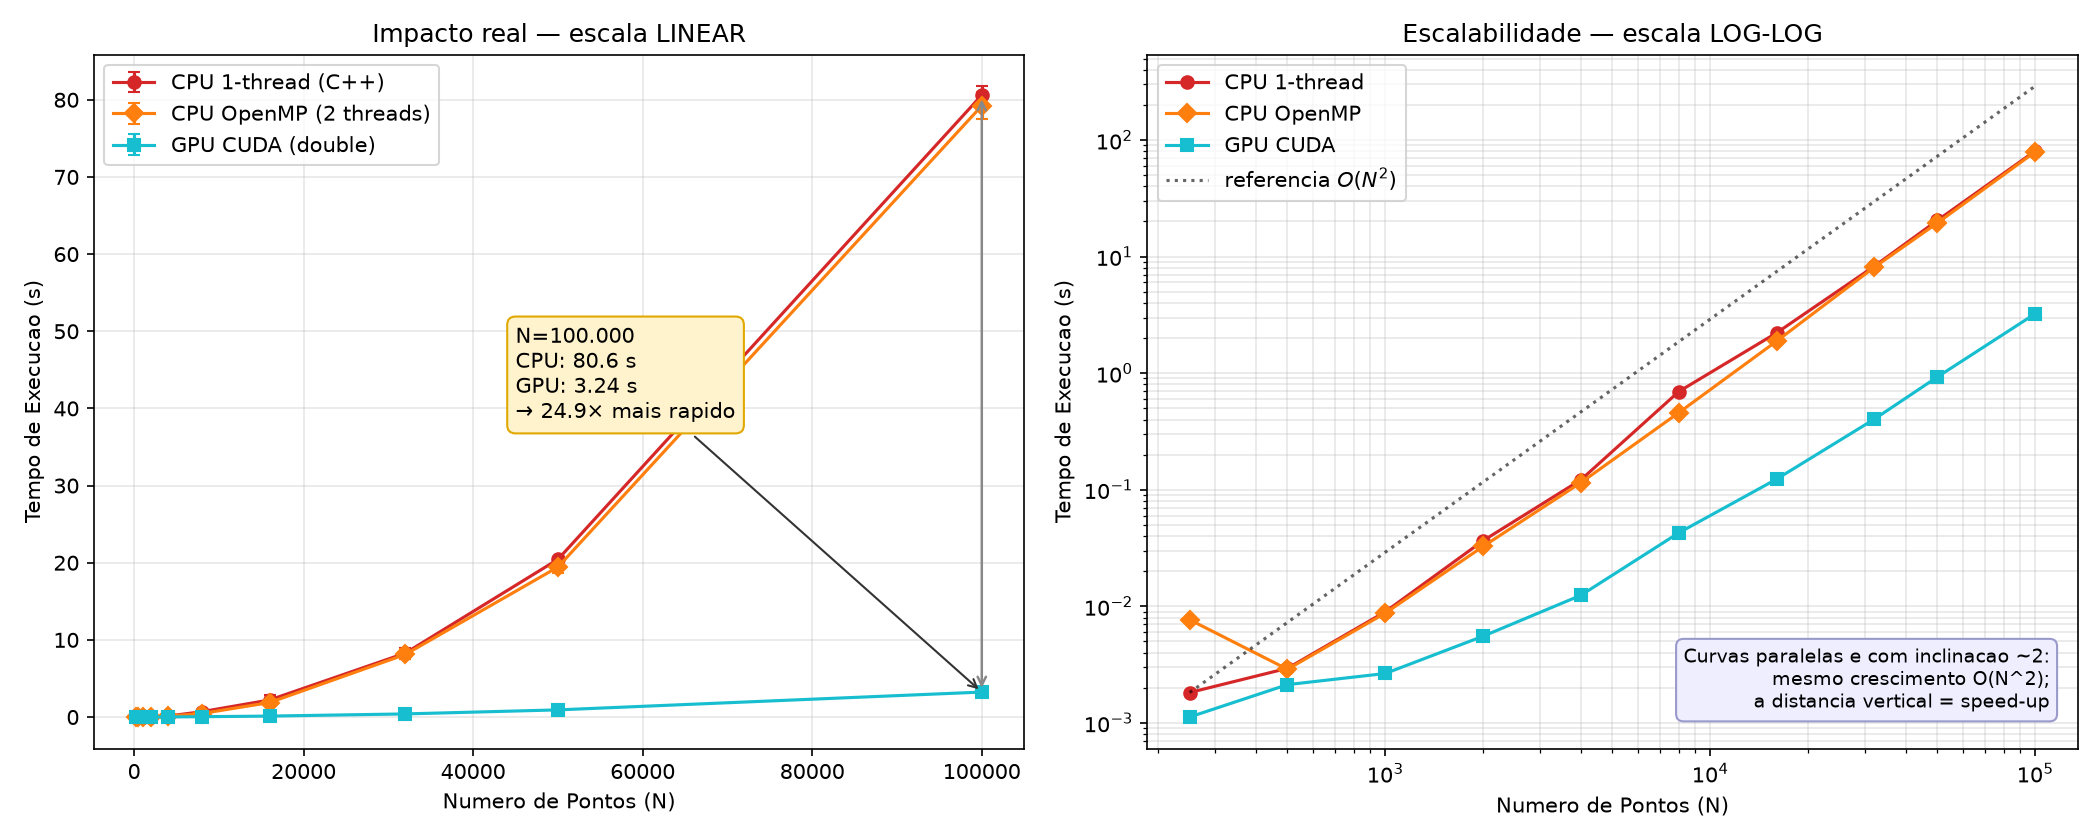
\includegraphics[width=\linewidth]{bench_tempo.png}
\caption{Tempo de execução \emph{vs.}\ $N$. Esquerda: escala linear, com o
\emph{gap} em $N=100.000$ destacado. Direita: escala log-log, com reta de
referência $O(N^2)$.}
\label{fig:tempo}
\end{figure}

A Figura~\ref{fig:speedup} apresenta o \emph{speed-up} em função de $N$
(eixo logarítmico). O ganho \textbf{cresce monotonicamente} com o tamanho do
problema: em $N$ pequeno, o custo fixo (inicialização e transferências)
domina e o \emph{speed-up} é modesto; à medida que o trabalho aumenta, esse
custo é amortizado. A anomalia em $N=250$ na curva OpenMP deve-se ao
\emph{overhead} de criação de \emph{threads} em problemas muito pequenos.

\begin{figure}[ht]
\centering
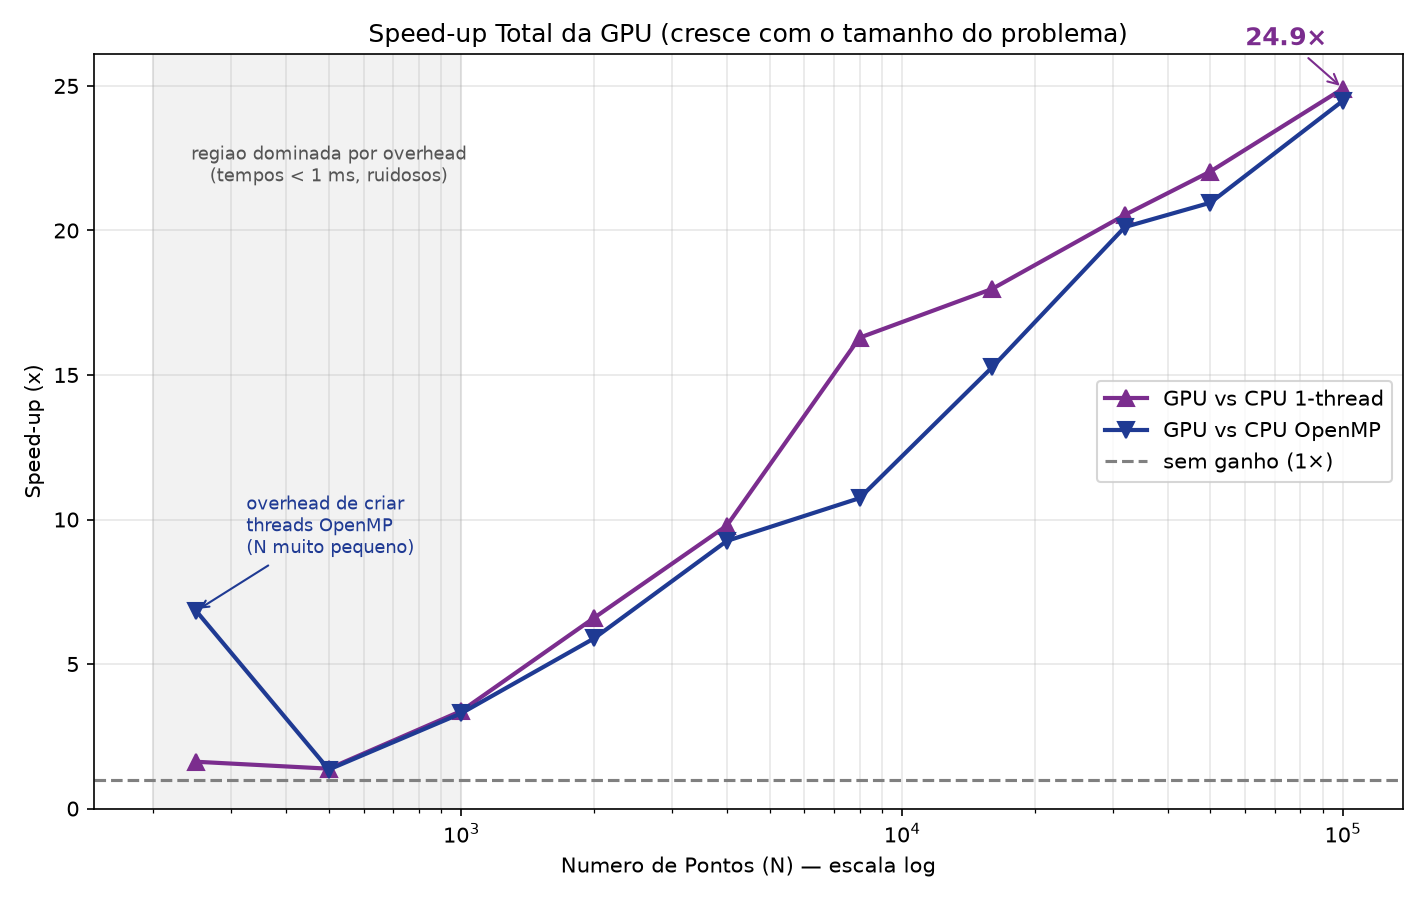
\includegraphics[width=0.85\linewidth]{bench_speedup.png}
\caption{\emph{Speed-up} da GPU em função de $N$ (eixo $N$ logarítmico),
contra a CPU sequencial e a CPU OpenMP.}
\label{fig:speedup}
\end{figure}

\subsection{Decomposição do tempo de GPU (\emph{breakdown})}
A Figura~\ref{fig:breakdown} decompõe o tempo de GPU por etapa. Dunn e
Silhueta --- as métricas que dependem de distâncias par-a-par ---
concentram \textbf{$\approx 99{,}95\%$} do tempo (em $N=100.000$,
$1{,}62$~s e $1{,}49$~s, respectivamente), enquanto Davies-Bouldin e a
transferência \emph{Host-to-Device} (H2D) são desprezíveis ($<0{,}001$~s).
Esse resultado tem implicação prática direta: como as transferências são
mínimas na formulação \emph{matrix-free}, técnicas de sobreposição de cópia
e computação (CUDA \emph{streams}) trariam ganho irrelevante neste caso ---
o problema é \emph{compute-bound}.

\begin{figure}[ht]
\centering
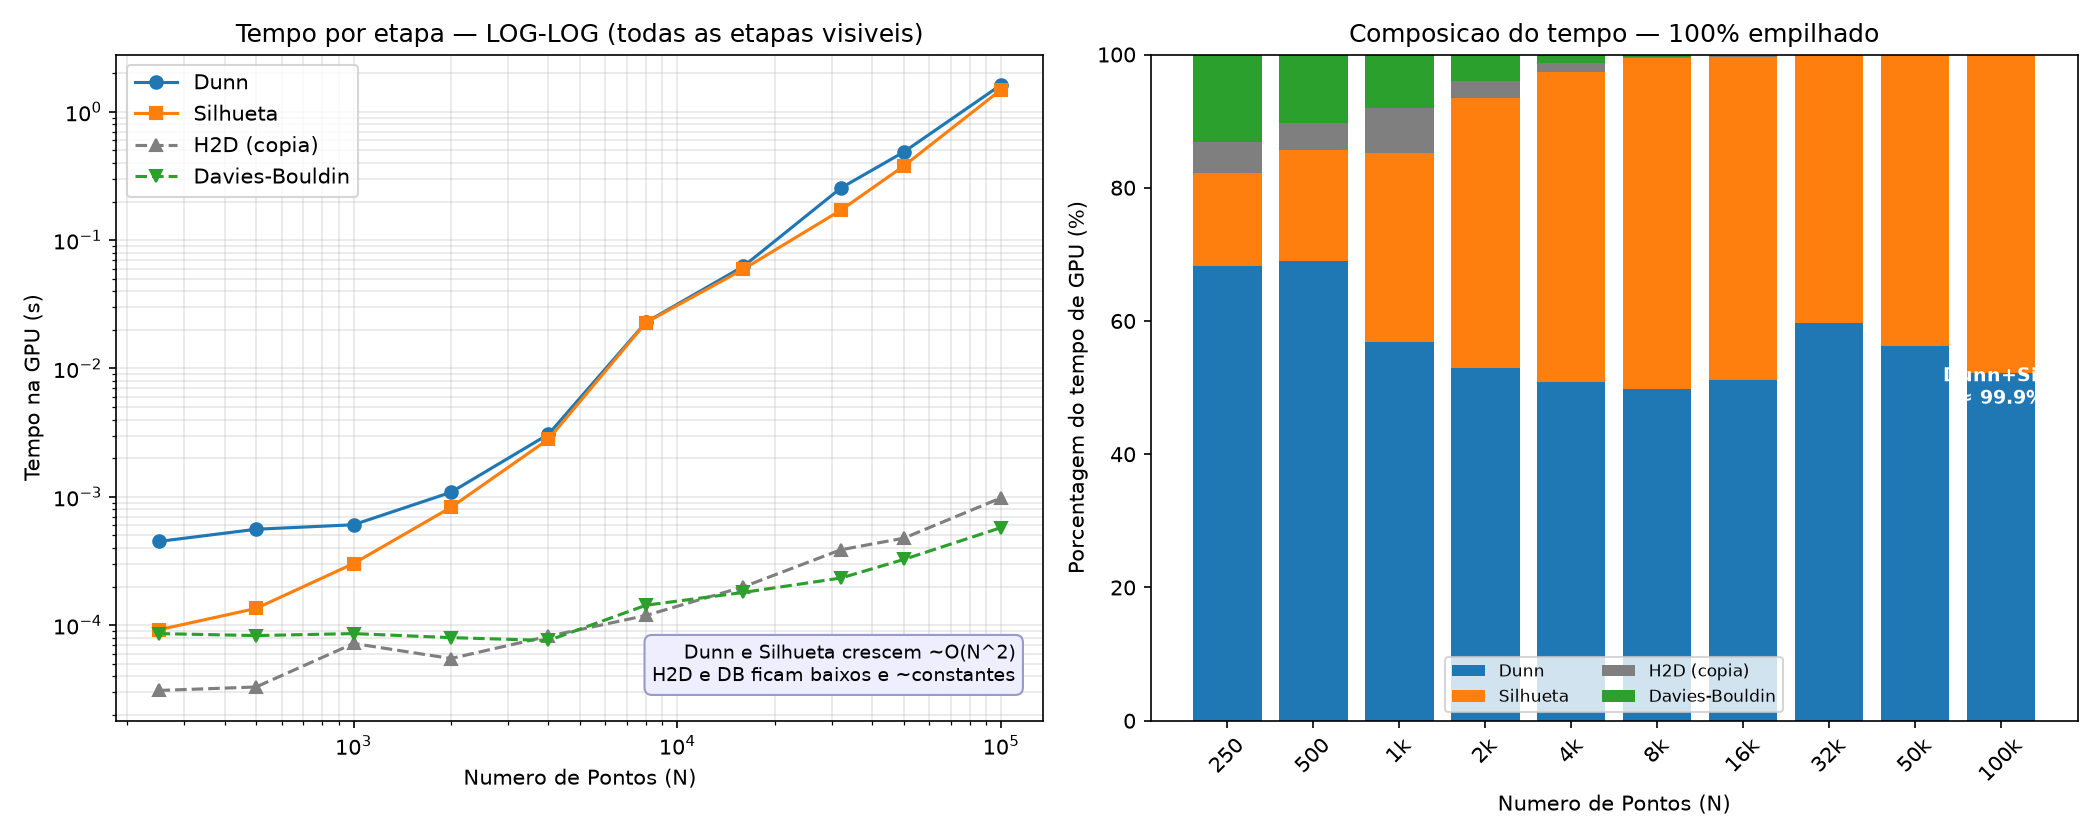
\includegraphics[width=\linewidth]{bench_breakdown.png}
\caption{Decomposição do tempo de GPU por etapa. Esquerda: escala log-log
(todas as etapas visíveis). Direita: composição percentual.}
\label{fig:breakdown}
\end{figure}

\subsection{Discussão}
Três aspectos merecem destaque. Primeiro, o \emph{speed-up} permanece
expressivo mesmo contra a \textbf{CPU paralela} (OpenMP), o que reforça a
validade científica do resultado --- não se trata de comparar a GPU apenas
com um único núcleo. Segundo, os ganhos são \textbf{conservadores}: a T4 é
particularmente fraca em precisão dupla, de modo que GPUs de maior porte
elevariam substancialmente o \emph{speed-up}. Terceiro, em relação ao
artigo-base~\cite{ncir2021}, nossa abordagem é \textbf{exata} (sem
amostragem) e executa em uma \textbf{única} GPU, sendo complementar à
estratégia distribuída e aproximada baseada em Spark: para volumes na casa
dos milhões, as duas ideias poderiam ser combinadas.

\subsection{Limitações}
Reconhecem-se as seguintes limitações: (i)~por ser \emph{matrix-free}, Dunn e
Silhueta \emph{recomputam} distâncias separadamente, o que um \emph{kernel}
fundido poderia evitar; (ii)~os experimentos usam dados sintéticos
bem-comportados (\emph{blobs}), sem clusters de formato irregular ou dados
reais; (iii)~o teto de $N=100.000$ é imposto pelo \emph{tempo} da CPU de
referência, não mais pela memória; (iv)~o \emph{kernel} de Silhueta usa
memória compartilhada proporcional a $K$, limitando $K$ muito elevados.

% ======================================================================
\section{Conclusão}
% ======================================================================

Este trabalho apresentou uma implementação paralela e \textbf{exata} em GPU
dos índices de Dunn, Silhueta e Davies-Bouldin para validação de
agrupamentos. A principal contribuição --- a estratégia \emph{matrix-free}
--- eliminou o gargalo de memória $O(N^2)$, reduzindo o consumo a
$O(N\cdot D)$ e viabilizando o processamento de até $100.000$ pontos, escala
inalcançável pela abordagem com matriz explícita. Mantendo corretude exata
(validada em três camadas independentes), obtivemos \emph{speed-up} de até
\textbf{24,9$\times$} sobre a CPU sequencial e \textbf{24,5$\times$} sobre a
CPU paralela (OpenMP), com o ganho crescendo com o tamanho do problema.

Como trabalhos futuros, destacam-se: a \textbf{fusão de \emph{kernels}} para
evitar a recomputação de distâncias; o uso de \textbf{múltiplas GPUs} e
precisão mista para alcançar a casa dos milhões de pontos; a combinação com
técnicas de \textbf{amostragem}~\cite{ncir2021} para validação aproximada em
\emph{big data}; e a avaliação sobre \emph{datasets} reais e com clusters de
formato arbitrário.

% ======================================================================
\begin{thebibliography}{9}

\bibitem{dunn1974}
DUNN, J. C.
\newblock Well-separated clusters and optimal fuzzy partitions.
\newblock \emph{Journal of Cybernetics}, v.~4, n.~1, p.~95--104, 1974.

\bibitem{rousseeuw1987}
ROUSSEEUW, P. J.
\newblock Silhouettes: a graphical aid to the interpretation and validation
of cluster analysis.
\newblock \emph{Journal of Computational and Applied Mathematics}, v.~20,
p.~53--65, 1987.

\bibitem{davies1979}
DAVIES, D. L.; BOULDIN, D. W.
\newblock A cluster separation measure.
\newblock \emph{IEEE Transactions on Pattern Analysis and Machine
Intelligence}, v. PAMI-1, n.~2, p.~224--227, 1979.

\bibitem{ncir2021}
NCIR, C. E. B.; HAMZA, A.; BOUAGUEL, W.
\newblock Parallel and scalable Dunn Index for the validation of big data
clusters.
\newblock \emph{Parallel Computing}, v.~102, 102751, 2021.

\bibitem{scikit2011}
PEDREGOSA, F. \emph{et al.}
\newblock Scikit-learn: Machine learning in Python.
\newblock \emph{Journal of Machine Learning Research}, v.~12, p.~2825--2830,
2011.

\bibitem{cuda}
NVIDIA.
\newblock \emph{CUDA C++ Programming Guide}.
\newblock NVIDIA Corporation, 2024.

\bibitem{openmp}
OPENMP ARCHITECTURE REVIEW BOARD.
\newblock \emph{OpenMP Application Programming Interface, Version 5.2}. 2021.

\end{thebibliography}

\end{document}
